\chapter{Desenvolupament del Projecte}

Com part important del projecte consta del disseny d'un nou llenguatge de programació, dedicaré una secció a explicar els principis de disseny i les característiques d'aquest llenguatge, de manera que les seccions posteriors siguin més entenadores.

En una segona secció, explicaré quins són els móduls del programa resultant i finalment entraré en detall als móduls més importants.

\section{Disseny}

Ja s'ha dit en la introducció quins punts de disseny seguirà el llenguatge, que s'anomena Quadriga en honor a un dels esports amb més renom disputats als Jocs Olímpics Clàssics, aqui parlarem de com s'ha tractat cada punt per, posteriorment, fer un resum de la seva estructura.

\begin{description}
  \item[Open Source] \hfill \\
    El codi del projecte s'ha penjat públicament a GoogleCode sota una llicència LGPL, que permet usar-la lliurement amb la única restricció d'haver de publicar els canvis fets sobre la mateixa llibreria sota la mateixa llicència. També s'ha optat per fer servir només llibreries OpenSource com el parsejador {\em JavaCC}, la llibreria gràfica {\em LWJGL} i la base de dades {\em HSQLDB}.
    
  \item[El sistema d'entitats ha de ser independent] \hfill \\
    S'ha optat per separar les {\em dades} de la funcionalitat, podent crear implementacions diferents per les mateixes dades, fent així que que fins hi tot poguem substituir totes les classes encarregades de renderitzar l'escena sense haver de tocar una línea de la definició de les entitats.
    
  \item[Ha de ser multi-plataforma de forma nativa] \hfill \\
    S'ha optat per programar sobre Java, i usar únicament llibreries escrites totalment amb Java o, en cas necessàri, amb codi natiu multiplataforma. S'intenta el màxim possible que no s'hagi de fer codi dependent de la plataforma.
    
  \item[Ha de permetre un desenvolupament ràpid un cop estiguin fets els components bàsics] \hfill \\
    S'ha intentat que la creació d'entitats i la seva interacció sigui el més senzilla possible.
    
  \item[Ha de ser fàcilment paral·lelitzable] \hfill \\
    S'han afegit expressament comportaments indefinits del programa, especialment en l'àmbit de l'ordre d'execució de certs elements, per exemple, d'ordre en que un sistema actualitza les entitats, o l'ordre en que 2 sistemes no relacionats s'actualitzen. D'aquesta manera es permet que el llenguatge mateix crei diferents fils d'execució i els balanceji de forma òptima.
\end{description}

\subsection{Definicions pròpies del llenguatge Quadriga}

\subsubsection{Entitat}

\subsubsection{Component}

\subsubsection{Sistema}

\subsubsection{Thread}

\subsubsection{Prototip}

\subsubsection{Main}

\section{Estructura del Programa}

\begin{figure}
  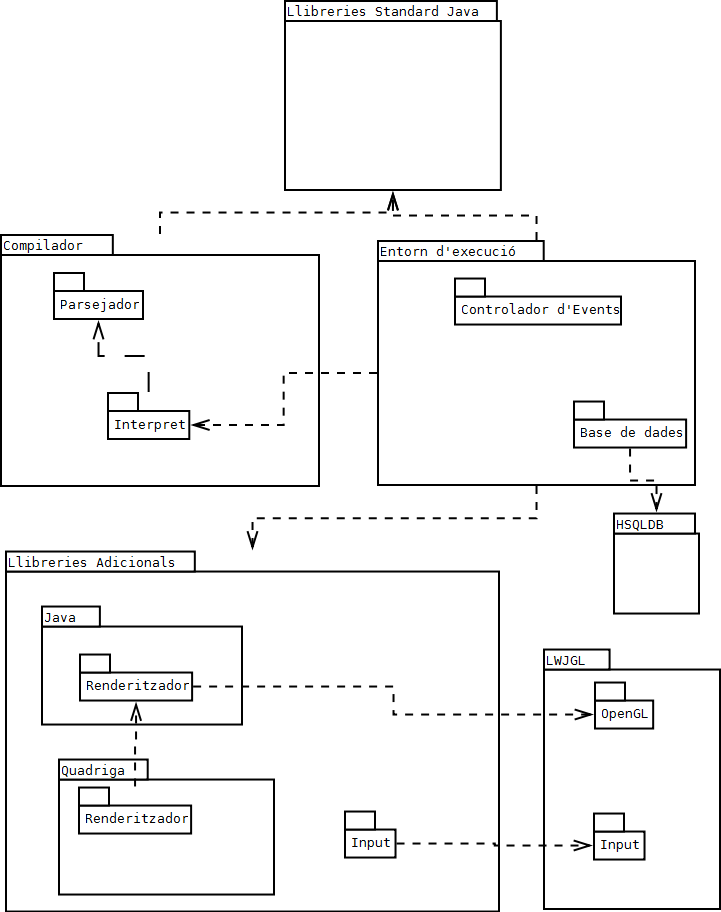
\includegraphics[width=1\linewidth]{./img/Moduls.png}
  \caption{Diagrama de móduls \label{fig:DiagramaDeModuls}}
\end{figure}

Com es veu a la figura \ref{fig:DiagramaDeModuls}, el programa consta d'un {\em compilador}, que a partir d'un seguit de fitxers crea una estructura de dades que posteriorment és interpretada. L'execució necessita d'un {\em entorn}, que s'encarrega essencialment de les operacions pròpies de {\em quadriga} com són la creació, destrucció i cerca de components i entitats, la relació d'un component amb una entitat, l'enviament d'events entre entitats o components, etc\ldots

\section{Model de Dades}